\chapter{Definicja węzła. Ruchy Reidemeistera}
Rozpoczynamy ten rozdział od sformułowania definicji węzła.
Obiekt, który zaraz określimy, powinien odpowiadać naszym oczekiwaniom, posiadać własności węzłów (żeby móc się tak nazywać), a przy tym zachowywać jak największy stopień ogólności.

Wydaje się, że poniższa definicja jest dosyć rozsądna.

\begin{definicja}
\label{zladefinicja}
	Węzłem nazywamy obraz gładkiej funkcji $f \colon \R \to \R^3$ o nieznikającej pochodnej, która posiada następującą własność: $f(u) = f(v)$ wtedy i tylko wtedy gdy $u - v \in \Z$.
\end{definicja}

Okazuje się jednak, że ma dość poważne wady.
Nie dopuszcza wprawdzie węzłów dzikich (rysunek poniżej), które posiadają nieskończenie wiele ,,pętli''.
Sprawia ona jednak kłopot w określeniu, kiedy dwa węzły są równoważne.
% 	\begin{center}
% 	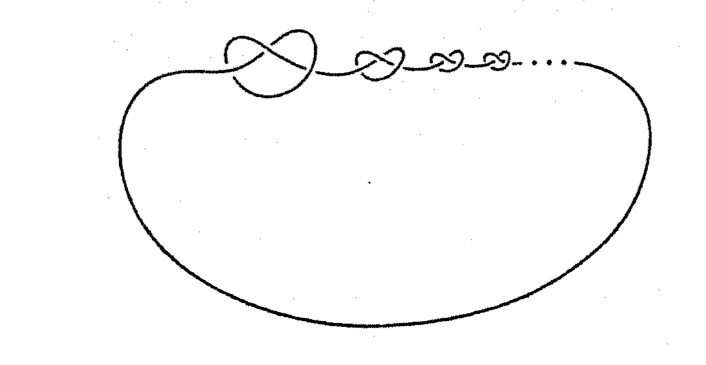
\includegraphics[scale=0.3]{1/pictures/wild.png}
% 	\end{center}
\begin{figure}[!ht]
	\centering
	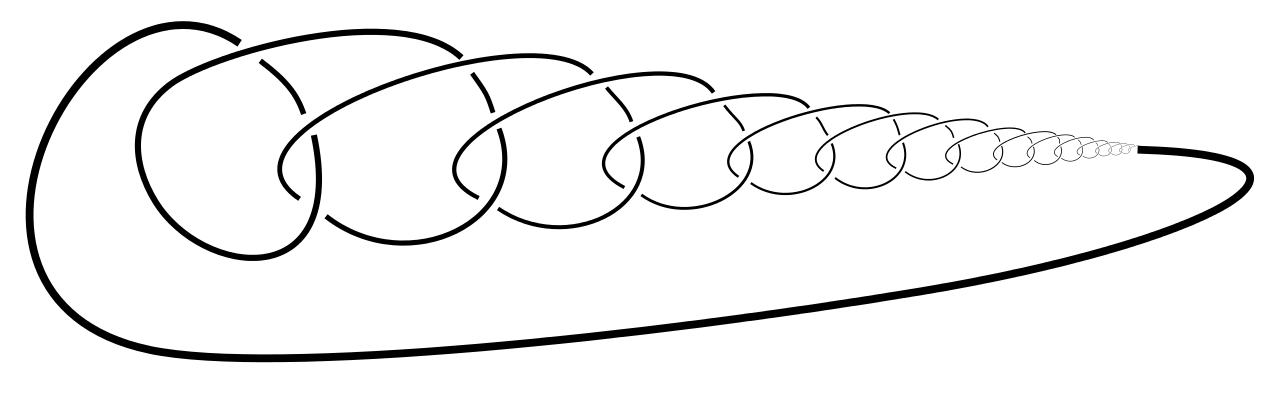
\includegraphics[scale=0.2]{img/wezeldziki.png}
	\caption{Węzeł dziki.}
	\label{fig:wezeldziki}
\end{figure}

Węzły $K$ i $J$ chcielibyśmy uważać za równoważne, jeżeli istnieje rodzina węzłów $K_t$ dla $t \in [0,1]$, taka że $K_0 = K$, $K_1 = J$ i $K_t$ powinien ,,nie różnić się'' znacznie od $K_s$ dla $s \approx t$.
Niestety umożliwia ona ściągnięcie każdej pętli do punktu.

\begin{figure}[!ht]
	\centering
	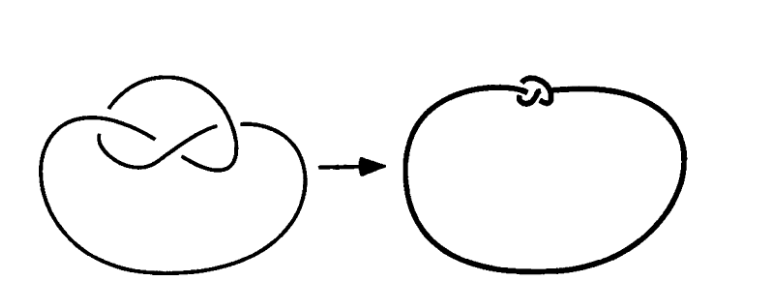
\includegraphics[scale=0.25]{img/petla.png}
	\caption{Ściągnięcie pętli.}
	\label{fig:wezeldziki}
\end{figure}

Rozwiązanie tych problemów jest zaskakująco proste: zamiast odwoływać się do pojęcia gładkiej krzywej, wystarczy posłużyć się łamaną.
Posiada ona skończenie wiele wierzchołków, więc wyklucza z rozważań dzikie węzły.
Pozwala również na podanie prostego opisu dozwolonych deformacji.

Skorzystamy z notacji $[p,q] := \{\lambda p + (1-\lambda)(q-p) : \lambda\in[0,1]\}$ dla różnych punktów $p, q \in \R^3$.
Łamaną o parami różnych wierzchołkach $p_1, \ldots, p_n \in \R^3$ jest zbiór $\bigcup_{i < n} [p_i, p_{i+1}]$.
Jeżeli $p_1 = p_n$, to łamana jest zamknięta.
Łamana jest pozbawiona samoprzecięć, kiedy każdy jej punkt naeży do dokładnie jednego odcinka postaci $[p_i, p_{i+1}]$.

\begin{definicja}
	Węzeł to łamana zamknięta w $\R^3$ bez samoprzecięć.
\end{definicja}

Zauważmy, że każdy węzeł jest jednoznacznie wyznaczony przez minimalny (w sensie zawierania) zbiór wierzchołków łamanej.

\begin{definicja}
	Splot to teoriomnogościowa suma skończenie wielu parami rozłącznych węzłów, zwanych składowymi.
\end{definicja}

\begin{przyklad}
Przykłady splotów: $\begin{tikzpicture}
	[x=0.705mm, y=0.75mm]
	\clip (-16,-10) rectangle (16,10);
	\foreach \r in {0,180}{
	\begin{scope}[rotate=\r]
		\path[TEXTARC, xshift=-13.5] (-32:9) arc (-32:300:9);
	\end{scope}}
\end{tikzpicture}$


\begin{minipage}[b]{0.24\linewidth}
\centering
\begin{tikzpicture}
	[x=0.75mm, y=0.75mm]
	\clip (-20,-10) rectangle (20,10);
	\draw[ARC] (-10,0) circle (9);
	\draw[ARC] (10,0) circle (9);
\end{tikzpicture}
\\
,,niesplot''
\end{minipage}
\begin{minipage}[b]{0.24\linewidth}
\centering
x
\\
splot Hopfa
\end{minipage}
\begin{minipage}[b]{0.24\linewidth}
\centering
\begin{tikzpicture}[x=1mm, y=1mm,]
\begin{scope}[scale=0.75]
	\clip (-17,-15) rectangle (17,15);
	\path[ARC] (-5,5) -- (5,-5);
	\foreach \r in {0,180} {
	\begin{scope}[rotate=\r]
		\path[ARC] (-8,8) .. controls (-20,20) and (-20,-20) .. (-1.5,-1.5);
		\path[ARC, rounded corners=15] (-6.5,-3.5) -- (-6.5,14) -- (6.5,14) -- (6.5,7.5);
	\end{scope}
	}
\end{scope}
\end{tikzpicture}
\\
splot Whiteheada
\end{minipage}
\begin{minipage}[b]{0.24\linewidth}
\centering
\begin{tikzpicture}[x=1mm, y=1mm,scale=0.75]
	\clip (-17,-14) rectangle (17,18);
	\foreach \r in {30,150,270}{
	\begin{scope}[rotate=\r]
		\path[ARC, xshift=-20] (-70:10) arc (-70:10:10);
		\path[ARC,xshift=-20] (35:10) arc (35:265:10);
	\end{scope}}
\end{tikzpicture}
\\
pierścienie Borromeuszy
\end{minipage}
\end{przyklad}

Zajmiemy się teraz utożsamianiem tylko pozornie różnych węzłów.

\begin{definicja}
\label{elementarne_p}
	O węźle $J$ rozpiętym na wierzchołkach $p_0, \ldots, p_n$ mówimy, że powstaje przez elementarną definicję węzła $K$ rozpiętego na $p_1, \ldots, p_n$, gdy $p_0$ nie leży na odcinku $[p_1, p_n]$, zaś przekrój trójkąta $p_0p_1p_n$ z $K$ zawiera się w $[p_1, p_n]$.
\end{definicja}

Przekształcenie odwrotne do elementarnej deformacji również jest elementarną deformacją.

% \begin{definicja}
%  Mówimy, że węzły $J$ i $K$ są równoważne, gdy istnieje skończony ciąg węzłów $K_0, K_1, \ldots, K_n$, gdzie $K_0$ = $K$, $K_n = J$, oraz $K_{i+1}$ jest elementarną
%  deformacją węzła $K_i$. 
% \end{definicja}

% Sprawdzenie, że podana relacja jest w istocie relacją równoważności pozostawiamy czytelnikowi jako proste ćwiczenie.

% Dla przykładu rozważmy dowolny $n$-kąt wypukły na płaszczyźnie. Można łatwo pokazać przez indukcję (po liczbie wierzchołków), że każdy taki wielokąt jest równoważny trójkątowi. 
% Istotnie, dla trójkąta
% teza jest oczywista. Załóżmy jej prawdziwość dla wszystkich liczb naturalnych nie większych, niż $n$. Mając dowolny $n+1$-kąt wypukły $J = (k_0, k_1, k_2, \ldots, k_n)$ łatwo się przekonać,
% że jest on elementarnym przekształceniem $n$-kąta $ K = (k_1, k_2, \ldots, k_n)$. To, że $K$ jest wielokątem wypukłym, podobnie jak to, że pierwszy warunek z definicji \ref{elementarne_p} jest spełniony, jest oczywiste.
% Drugi warunek jest spełniony, ponieważ z wypukłości $K$ zachodzi $\left([p_0,p_1]\cup [p_0, p_n]\right) \cap K = \lbrace p_1, p_n\rbrace$.

% \begin{definicja}
%  Każdy węzeł, który jest elementem klasy abstrakcji opisanej w przykładzie nazywamy niewęzłem.
% \end{definicja}
% \begin{definicja}
%  Sploten trywialnym nazywamy sumę mnogościową skończenie wielu rozłącznych niewęzłów leżących w jednej płaszczyźnie.
% \end{definicja}

% \textbf{Uwaga} W przypadku nie-splotu warunek leżenia w jednej płaszczyźnie jest istotny. Aby się o tym przekonać czytelnik może zechcieć odpowiedzieć na pytanie, 
% jak mogą leżeć względem siebie rozłączne okręgi w $\mathbb{R}^3$, a jak muszą w $\mathbb{R}^2$.

% Od tej chwili węzły równoważne będziemy uważać za tożsame, to znaczy zamiast pisać, że węzeł $J$ jest równoważny węzłowi $K$, będziemy pisać krótko $J=K$ (właśnie w taki sposób
% został powyżej zdefiniowany niewęzeł).
% Odróżniać będziemy tylko te węzły, które nie są równoważne. 

% \subsection{Diagram}
% Od początku tej pracy, z konieczności rysowaliśmy węzły (obiekty żyjące w przestrzeni trójwymiarowej) na płaszczyźnie. 
% W tym podrozdziale podamy ścisłą definicję tych dwuwymiarowych rysunków (diagramów) i pokażemy, że jeśli dwa węzły mają przedstawienie w postaci tego samego diagramu, 
% to są w istocie równoważne.

% \begin{definicja}
%  Rzutem zbioru $A\subseteq\mathbb{R}^3$ na płaszczyznę nazwiemy funkcję $p\colon A\to\mathbb{R}^2$ określoną wzorem $p(x,y,z) = (x,y)$. Kiedy $A$ jest węzłem, $p[A]$ nazywamy 
%  rzutem węzła $A$ na płaszczyznę.
% \end{definicja}


% \begin{definicja}
% \label{rzut_reg}
%  Rzutem regularnym węzła $K$ nazywamy takie rzutowanie $p$ węzła $K$ na płaszczyznę, że
%  \begin{enumerate}
%   \item dla każdego wierzchołka $v$, dla każdego $a\in K$ jeśli $p(v) = p(a)$, to $p=a$,
%   \item dla każdych $a_1, a_2, a_3$ jeśli $p(a_1)=p(a_2)=p(a_3)$, to $a_1=a_2$ lub $a_1=a_3$ lub $a_2=a_3$.
%  \end{enumerate}
% \end{definicja}

% Zakładająć, że węzeł ma regularny rzut na płaszczyznę, możemy w ścisły sposób zdefiniować pojęcie diagramu.
% Diagramem węzła $K$ nazywamy następującą modyfikację regularnego rzutu $K$ na płaszczyznę. Jeśli przeciwobrazem punktu $(x_0, y_0)$ jest zbiór dwuelementowy 
% $\lbrace a,b\rbrace$, wówczas w tym punkcie przecinają się dwa różne odcinki, które są rzutami dwóch różnych odcinków węzła $K$, powiedzmy $I_a, I_b$. 
% Ponieważ rzut $K$ jest rzutem regularnym, więc jeden z tych odcinków leży pod drugim, co oznaczamy, jak na poniższym rysunku. \\


% 	\begin{center}

% 	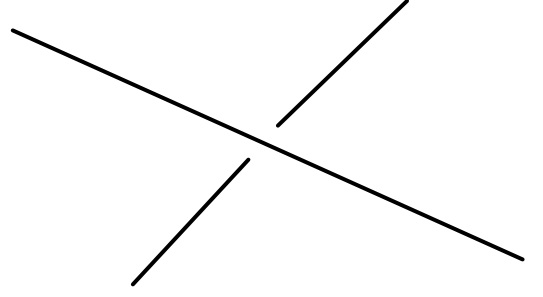
\includegraphics[scale=0.4]{1/pictures/skrz.jpg}
% 	\end{center}


% \begin{definicja}
%  Mówimy, że dwa węzły $(p_i)$, $(q_j)$ są od siebie odległe o mniej, niż $t$, gdy mają tyle samo wierzchołków i gdy dla każdej pary wierzchołków zachodzi $d(p_k,q_k) < t$.
% \end{definicja}

% Udowodnimy teraz twierdzenie, które zagwarantuje nam, że dla każdego węzła można znaleźć węzeł dowolnie mu bliski, który jest równoważny z wyjściowym, i którego rzut na płaszczyznę jest regularny. 
% Będziemy do tego potrzebować następujących lematów.

% \begin{lemat}
% \label{LEM1}
%  Dla dowolnego węzła $K = (v_0, \ldots, v_i, \ldots, v_n)$ i dowolnego $i\in\lbrace 1,2,\ldots n\rbrace$ istnieje taki $\epsilon > 0$, że dla każdego $v'\in B(v_i, \epsilon)$ 
%  węzły $K$ oraz $(v_0, \ldots,v_{i-1}, v', v_{i+1}, \ldots, v_n)$ są równoważne.
% \end{lemat}
% \begin{proof}

% Ustalmy dowolne $i$. Dodawanie i odejmowanie indeksów w dalszej części dowodu należy rozumieć jak działanie modulo $n+1$. Możemy założyć, że punkty $v_{i-1}, v_i, v_{i+1}$ nie są
% współliniowe. Zaczniemy dowód od skonstruowania dwóch stożków.
% Stożek o wierzchołku $w$, środku podstawy $s$ i promieniu podstawy $r$ będę oznaczał $S(s,r,w)$. 

% Niech $p\in\mathbb{R}^3$ będzie wektorem długości jeden prostopadłym do odcinków $I_{i-1}$ oraz $I_i$. Oznaczmy przez $\alpha$ kąt pomiędzy odcinkami 
% $I_{i-2}$ i $I_{i-1}$. 
% Dobierzmy tak małą $\mu\in\mathbb{R}^3$, żeby kąt pomiędzy $I_{i-1}$ oraz $[v_{i-1}, v_i + \mu p]$ był mniejszy od $\alpha$. Możemy $\mu$ wyliczyć np. używając trygonometrii 
% w trójkącie prostokątnym o wierzchołkach $v_{i-1}, v_i, v_i + r\cdot p$, gdzie $r\in\mathbb{R}_+$. Połóżmy
% \begin{displaymath}
%  \epsilon = \frac{1}{2}\min\lbrace d(I_{i-1}, K\setminus(I_{i-2}\cup I_i)), \mu\rbrace, \hbox{ oczywiście }\epsilon>0.
% \end{displaymath}
% Wtedy
% \begin{enumerate}
%  \item $S(v_i, \epsilon, v_{i-1})\cap K \subseteq I_{i-1}\cup I_i$,
%  \item dla każdej $\delta\in(0,\epsilon)$ zachodzi $[v_{i-1}, v_i+\delta p]\subseteq S(v_i, \epsilon, v_{i-1})$.
% \end{enumerate}
% Zauważmy, że $d(v_i, cl(K\setminus(I_{i-1}\cup I_i)) > 0$, więc (jako że $\mathbb{R}^3$ jest $T_4$) można znaleźć takie
% $\gamma > 0$, że $B(v_i,\gamma)\cap cl(K\setminus(I_{i-1}\cup I_i)) = \emptyset$. Możemy wziąć takie $\gamma$, żeby $\gamma < \epsilon$.

% Wtedy stożek 
% $S_{i-1} = S(v_i + \gamma(v_i-v_{i-1}), \epsilon, v_{i-1})$ spełnia własność $1$ oraz własność
% \begin{displaymath}
%  \hbox{dla każdego }v'\in B(v_i, \gamma) \ \ [v_{i-1}, v']\subseteq S_{i-1}.
% \end{displaymath}


% W analogiczny sposób konstruujemy stożek $S_i = S(v_i + \gamma'(v_i - v_{i+1}), \epsilon', v_{i+1})$. Zbiory $S_{i-1}$ i $S_i$ mają niepuste wnętrza, oraz 
% $v_i\in int(S_i)\cap int(S_{i+1})$. Istnieje więc taka liczba $r>0$, że $B(v_i, r)\subseteq S_i\cap S_{i+1}$.

% Owe stożki pomogą nam pokazać, że dla każdego $v'\in B(v_i, r)$ węzeł $(v_1, \ldots, v', \ldots, v_n)$ jest równoważny $K$.

% Ustalmy $v'\in B(v_i, r)$. Wtedy odcinki $[v_{i-1}, v'], [v',v_i], [v', v_{i+1}]$ należą do zbioru $S_i\cup S_{i-1}$, który jest rozłączny z $K\setminus(I_{i-1}\cup I_i)$. 
% Rozważmy dwa przypadki. 

% Jeżeli $v'\in I_i$ (gdy $v'\in I_{i-1}$, to postępujemy analogicznie), to węzeł $K$ można zdefiniować za pomocą łamanej $(v_1, \ldots, v_i, v', v_{i+1}, \ldots, v_n)$. Ponieważ
% wnętrze odcinka $[v_{i-1}, v']$ jest rozłączne z $K$, więc $K$ jest równoważny węzłowi $(v_1, \ldots, v_{i-1}, v', v_{i+1}, \ldots, v_n)$.

% Jeśli $v'\not\in I_i\cup I_{i-1}$, wówczas wnętrze odcinka $[v_i, v']$ jest rozłączne z $I_i\cup I_{i-1}$. Rozważmy odcinek $[v_{i-1}, v']$, jeśli przecina on odcinek $I_i$, to 
% wtedy odcinek $[v', v_i]$ nie przecina odcinka $I_{i-1}$, zatem bez zmniejszenia ogólności możemy założyć, że wnętrze odcinka $[v_{i-1}, v']$ jest rozłączne z $K$. Tworzymy
% następujący ciąg
% \begin{displaymath}
%  K_0 = K, K_1 = (v_1,\ldots, v_{i-1}, v', v_i, \ldots, v_n), K_2 = (v_1,\ldots, v_{i-1}, v', v_{i+1}, \ldots, v_n).
% \end{displaymath}
% Czytelnik zechce się sam przekonać, że jest to ciąg elementarnych deformacji. 
% Kładziemy $K' = K_2$ i kończymy dowód.
% \end{proof}
% \textbf{Uwaga} Ponieważ funkcja
%  $ d(x,y)\mapsto d(p(x), p(y))$ jest nierosnąca, więc przy oznaczeniach, jak w dowodzie lematu zachodzi $p(v')\in B(p(v_i),\epsilon)$.

% \begin{lemat}
%  \label{LEM2}
%  Rozpatrzmy węzeł $K = (v_1, \ldots, v_n)$. Niech $p$ oznacza rzut na płaszczyznę. Dla każdego $i$, dla każdego $\epsilon > 0$ istnieje węzeł
%  węzeł $J = (q_1, \ldots, q_i, \ldots q_n)$ równoważny węzłowi $K$ odległy od $K$ o mniej niż $\epsilon$ oraz spełniający:
%  dla dowolnego $r\in J$ i dla dowolnego $i$ zachodzi $p(q_i)\neq p(r)$, gdzie $p$ oznacza rzut prostokątny na płaszczyznę $OXY$.
% \end{lemat}
%  \begin{proof}
%   Niech $i$ będzie dowolne. 
%   Niech $\epsilon'$ będzie dobrany do wierzchołka $v_i$, jak w tezie lematu \ref{LEM1}. W razie potrzeby możemy go zmniejszyć, tak by $\epsilon'<\epsilon$. 
%   Zauważmy, że $p[B(v_i, \epsilon')] = B(p(v_i),\epsilon')$, gdzie kula po lewej stronie równości jest z $\mathbb{R}^3$, a po prawej z $\mathbb{R}^2$. Ponieważ zbiór $p(K)$ jest nigdziegęstym podzbiorem płaszczyzny, więc możemy wybrać taki $q_i\in B(v_i, \epsilon')$,
%   że $p[\lbrace q_i\rbrace]\cap p[K] = \emptyset$. Otrzymujemy w ten sposób nowy węzeł $(v_1, \ldots, q_i, \ldots, v_n)$. Powtarzamy opisaną procedurę $n-1$ razy i w efekcie 
%   otrzymujemy węzeł $J$. Ponieważ $\epsilon'$ był z lematu \ref{LEM1}, więc $J$ i $K$ są równoważne. 
%  \end{proof}


% \begin{twierdzenie}
%  Niech $K$ będzie węzłem o uporządkowanym zbiorze wierzchołków $(v_1, v_2, \ldots, v_n)$. Dla każdego $\epsilon > 0$ istnieje węzeł $K'$, 
% który jest odległy od węzła $K$ o nie więcej, niż $\epsilon$, oraz jego rzut na płaszczyznę $OXY$ jest regularny. 
% \end{twierdzenie}
% \begin{proof}

% Najpierw zastosujemy lemat \ref{LEM2} do węzła $K$ i powstały w ten sposób węzeł oznaczymy przez $K'$.

% Ponieważ rzut węzła $K'$ spełnia pierwszy warunek z definicji \ref{rzut_reg}, więc dla dwóch różnych odcinków $I,J$ węzła 
% $K'$ zachodzi $|p(I)\cap p(J)| \le 1$.

% Niech $\mathcal{A}$ będzie rodziną wszystkich takich podzbiorów zbioru odcinków węzła $K'$, że dla każdego $A\in\mathcal{A}$ zachodzi 
% \begin{enumerate}
%  \item $|A| > 1$,
%  \item istnieje taki $r\in\mathbb{R}^2$, że $\bigcap_{I\in A}p(I) = \lbrace r\rbrace$,
%  \item dla każdego $J\not\in A$ $\left(\bigcap_{I\in A}p(I)\right)\cap p(J) = \emptyset$.
% \end{enumerate}

% Niech $a\in K'$ będzie punktem z wnętrza pewnego odcinka $I_i$, takim że istnieją różne od $a$ punkty $b, c\in K'$ takie że $p(a) = p(b) = p(c)$ i $b\neq c$. 
% Niech $\lbrace t_A\rbrace_{A\in\mathcal{A}}$ będzie ciągiem w $\mathbb{R}^2$, takim że $t_A = \bigcap_{I\in A}p(I)$. Niech $u\in\mathbb{R}^2$ będzie niezerowym wektorem prostopadłym do osi $OZ$, który
% nie jest równoległy do $p(I_{i-1})$ oraz nie jest równoległy do $p(I_{i+1})$. Wtedy, używając tego samego argumentu, co w dowodzie lematu \ref{LEM2}, możemy znaleźć dostatecznie małą $\delta > 0$, że dla każdej $0 < \delta' < \delta$ istnieje wektor $w$, taki że
% węzeł $(v_1, \ldots, v_{i-1}, v_i  + \delta'w, v_{i+1}  + \delta'w, v_{i+2}, \ldots, v_n)$ jest równoważny węzłowi $K'$, oraz rzut tego węzła spełnia punkt pierwszy 
% defnicji \ref{rzut_reg}. Ponieważ ciąg $t_A$ jest skończony, to
% liczbę $\delta'$ można wziąć na tyle małą, żeby była mniejsza od dowolnej dodatniej odległości $d(p(I_j), t_A)$ dla $j \in \lbrace i-1, i+1\rbrace$.
% Wtedy węzeł powstały z $K'$ przez zastąpienie $v_i, v_{i+1}$ wierzchołkami $v_i'=v_{i} + \delta'w, v_{i+1}'=v_{i+1}+\delta'w$
% odpowiednio jest równoważny węzłowi $K'$, co więcej, dla każdego $r\in[v_{i-1}, v_i']\cup[v_i', v_{i+1}']\cup[v_{i+1}', v_{i+2}]$ istnieje co najwyżej jeden taki $r'\neq r$, że $p(r') = p(r)$.
% Zauważmy, że po tej zastosowaniu tej procedury przynajmniej jeden element rodziny $\mathcal{A}$ ma jeden element mniej.
% zatem w skończonej liczbie kroków dojdziemy do momentu, kiedy w rodzinie $\mathcal{A}$ zostaną jedynie zbiory dwuelementowe. Wtedy rzut otrzymanego węzła będzie regularny. 

% \end{proof}


% Warto podkreślić, że dwa różne węzły (w sensie relacji równości) mogą mieć ten sam diagram, np. mając dany węzeł można przesunąć jego wierzchołek o największej trzeciej współrzędnej 
% o wersor równoległy do osi $OZ$. Okazuje się jednak, że jeśli dwa węzły mają ten sam diagram, to są równoważne. 


% \begin{twierdzenie}
%  Jeśli dwa węzły $K = (v_1,\ldots, v_n)$ oraz $W = (w_1, \ldots, w_n)$ mają regularne rzutowanie oraz ich diagramy są równe, to $K$ i $J$ są równoważne.
% \end{twierdzenie}
% \begin{proof}
%  Ustalmy wierzchołek $v_i$. Zauważmy, że bez straty ogólności możemy założyć, że rzut każdego z odcinków $I_i, I_{i-1}$ węzła $K$ zawiera co najwyżej jedno skrzyżowanie. 
%  Istotnie, jeśli
%  rzut odcinka $I_i$ zawiera więcej skrzyżowań (oczywiście jest ich skończenie wiele), to niech $s_0$ oznacza skrzyżowanie najbliższe $p(v_i)$, a $s_1$ skrzyżowanie najbliższe
%  punktowi $s_0$. Wybierzmy dowolny punkt z wnętrza odcinka $[s_0, s_1]$, oznaczmy go przez $s$. Niech $v' = p^{-1}(s)$. Wtedy łamana $(v_1, \ldots, v_i, v', v_{i+1})$ definiuje 
%  węzeł $K$. Wówczas odcinek $p[ [v_i, v']]$ zawiera dokładnie jedno skrzyżowanie. To samo możemy założyć o węźle $J$ dodając nowy wierzchołek $q'$ w punkcie $p^{-1}(s)$.
 
%  Niech $I, J$ oznaczają te odcinki węzła $K$, że $p[I]\cap p[I_i]\neq\emptyset$ oraz $p[J]\cap p[I_{i-1}]\neq\emptyset$. Wtedy $I$ leży ,,pod'' odcinkiem $I_i$ i pod odcinkiem
%  węzła $W$, który jest rzutowany na $p[I_i]$, albo ,,nad'' oboma tymi odcinkami. To samo się tyczy odcinka $J$. Stąd wynika, że wnętrza odcinków $[v_{i-1}, w_i], [w_i, v_{i+1}]$ są
%  rozłączne z węzłem $K$. To, że $K\cap [v_i,w_i] = \lbrace v_i\rbrace$ jest oczywiste. Dlatego ciąg
%  \begin{displaymath}
%   K_0 = (v_1, \ldots, v_n), K_1 = (v_1, \ldots, v_{i-1}, w_i, v_i, v_{i+1}, \ldots, v_n), K_3 = (v_1, \ldots, v_{i-1}, w_i, v_{i+1}, \ldots, v_n)
%  \end{displaymath}
% jest ciągiem elementarnych deformacji. Stosując powyżej opisaną procedurę do każdego wierzchołka węzła $K$ otrzymamy na końcu węzeł $J$, co znaczy, że te węzły są równoważne.
 
%  \end{proof}

% \subsection{Każdy kij ma dwa końce, czyli orientacja węzła}
% Jak już wcześniej zostało powiedziane, węzeł to łamana w $\mathbb{R}^3$. Łamana z kolei jest wyznaczona jednoznacznie przez zbiór  swoich wierzchołków. Mając dany węzeł o wierzchołkach
% $(v_1, v_2, \ldots, v_n)$, możemy go zorientować, to znaczy dla każdego odcinka węzła wybrać początek i koniec tego odcinka. Chcielibyśmy to zrobić w taki sposób, żeby każdy wierzchołek
% był końcem dokładnie jednego odcinka. W tym sensie węzeł $(v_1, v_2, \ldots, v_n)$ jest węzłem różnym od węzła $(v_n, \ldots, v_2, v_1)$, mimo, że jako podzbiory $\mathbb{R}^3$ są
% sobie równe. Teraz spróbujemy sformalizować to, co dotychczas powiedzieliśmy.

% \begin{definicja}
%  Odcinkiem zorientowanym w $\mathbb{R}^3$ o początku w $p$ i końcu w $q$ (zakładamy, że $p\neq q$) nazywamy liniowe włożenie $l\colon[0,1]\to\mathbb{R}^3$, takie że $l(0) = p, l(1) = q$ i oznaczamy przez
%  $[p,q]_o$. 
% \end{definicja}

% Innymi słowy odcinek zorientowany to odcinek z wyróżnionym początkiem i końcem. Co więcej, przy oznaczeniach z definicji zachodzi
% \begin{displaymath}
%  q-p =  |q-p|\cdot\frac{l'(x)}{|l'(x)|}, \hbox{ dla dowolnego } 0 < x < 1.
% \end{displaymath}

% \begin{definicja}
%  Orientacją węzła $K = (v_1, v_2, \ldots, v_n)$ nazywamy takie zorientowanie jego odcinków, że każdy wierzchołek jest końcem (równoważnie - początkiem) dokładnie jednego odcinka.
% \end{definicja}

% Nie trudno się przekonać, że każdy węzeł można zorientować na dokładnie dwa sposoby. Istotnie, wybranie orientacji jednego odcinka węzła jednoznacznie wyznacza orientacje całego
% węzła. 

% Przyjmiemy następującą konwencję, jeśli powiemy, że węzeł $K = (v_1, v_2, \ldots, v_n)$ jest węzłem zorientowanym, będziemy przez to rozumieć, że $I_1 = [v_1, v_2]_o$.

% \textbf{Uwaga} Niech będzie dany węzeł $K = (v_1, v_2, \ldots, v_n)$, niech ponadto uporządkowane $n$-tki $K_i = (v_{i_1}, v_{i_2}, \ldots, v_{i_n})$ 
% oraz $K_j = (v_{j_1}, v_{j_2}, \ldots, v_{j_n})$ definiują ten sam węzeł $K$. Niech $O_i, O_j$ oznaczają orientację zorientowanych węzłów $K_i, K_j$ odpowiednio. Powiemy, że orientacja
% $O_i$ jest równoważna orientacji $O_j$, gdy isnieje taka $\sigma\in S_n$, że dla każdego $k$ zachodzi $\sigma(i_k) = j_k$. Sprawdzenie, że ta relacja jest w istocie relacją równoważności
% pozostawiamy jako proste ćwiczenie. 

% \begin{definicja}
%  Węzłem zorientowanym nazywamy węzeł z wybraną orientacją.
% \end{definicja}

% Elementarne deformacje węzła zorientowanego definiuje się w sposób oczywisty. Do zestawu punktów $(1), (2)$ z definicji \ref{elementarne_p} należy dodać następujący warunek.
% \begin{displaymath}
%  \hbox{Odcinki zorientowane koincydentne z wierzchołkiem } p_0 \hbox{ są równe }[p_n, p_0]_o, [p_0, p_1]_o.
% \end{displaymath}

% \begin{definicja}
%  Węzły zorientowane nazywamy równoważnie zorientowanymi, gdy w skończenie wielu krokach za pomocą elementarnych deformacji jednego węzła zorientowanego
%  możemy otrzymać drugi.
% \end{definicja}
% Należy wyraźnie powiedzieć, że równoważność dwóch węzłów jest istotnie inną relacją, niż równoważność węzłów w sensie orientacji. Istnieją bowiem przykłady węzłów równoważnych
% ale nie równoważnych w sensie orientacji. Opisanie ich dokładnie wykracza jednak poza możliwości intelektualne autora, dlatego fakt ten, z wyższej konieczności, jest podany
% czysto informacyjnie. 
% Na koniec tego rozdziału podamy jeszcze jedną definicję.
% \begin{definicja}
%  Odwrotnością węzła zorientowanego $K = (v_1, v_2, \ldots, v_n)$ nazywamy węzeł $K^r = (v_n, v_{n-1}, \ldots, v_1)$. Powiemy, że $K$ jest węzłem odwracalnym, jeżeli $K$ i $K^r$ są
%  równoważne w sensie orientacji. Dla węzła $J$ niezorientowanego, powiemy że jest on odwracalny, jeśli istnieje taka orientacja węzła $J$, że jest on odwracalny (jako węzeł
%  zorientowany z tą wybraną orientacją).
% \end{definicja}


% \subsection{Ruchy Reidemeistera}
% W tym podrozdziale przedstawimy pierwsze poważne narzędzie, które w wielu przypadkach pozwoli nam rozstrzygnąć, czy dwa węzły są równoważne, czy też nie. 
% Na początku sformuujemy nową definicję elementarnej deformacji, równoważną tej, którą wpprowadziliśmy wcześniej.

% \begin{definicja}
% \label{wygoda}
%  Węzeł $K'$ jest elementarną deformacją węzła $K = (v_1,, v_2, \ldots, v_n)$, gdy
%  \begin{enumerate}
%   \item $K'=(v_1, v_2, \ldots, v_i, v', v_{i+1}, \ldots, v_n)$, gdzie $v'\in \hbox{Int}I_i$, lub
%   \item $K' = (v_1, v_2, \ldots, v_{i-1}, v', v_{i+1}, \ldots, v_n)$, o ile czworokąt $C$ o wierzchołkach $v_{i-1}, v_i, v_{i+1}, v'$ spełnia $C\cap K = I_{i-1}\cup I_i$.
%  \end{enumerate}
%  Równoważność tej definicji z definicją podaną wcześniej jest oczywista.
% \end{definicja}

% \begin{definicja}
%  Następujące trzy operacje (wraz z operacjami odwrotnymi - w sumie jest ich sześć) nazywamy ruchami Reidemaistera.
 
% 	\begin{enumerate} 

% \item Pierwszy ruch Reidemeistera: 
	
% 	\begin{minipage}{0.5\textwidth}
% 		\begin{center}
% 			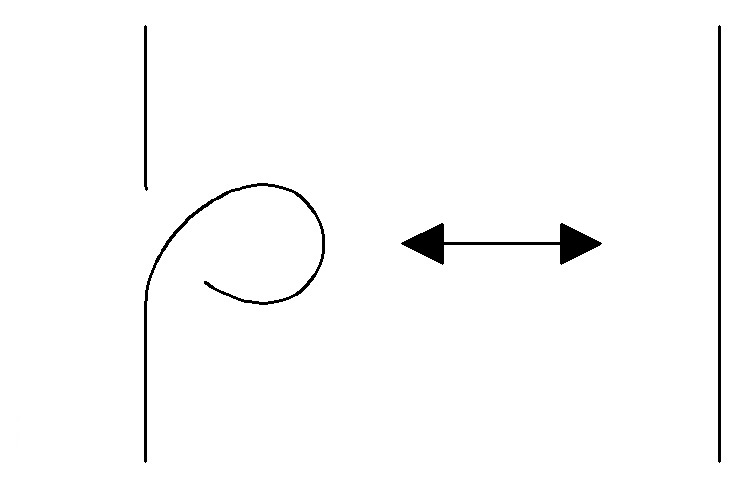
\includegraphics[scale=0.2]{1/pictures/R1}
% 		\end{center}
% 	\end{minipage}
% \item Drugi ruch Reidemeistera: 

% 	\begin{minipage}{0.5\textwidth}
% 		\begin{center}
% 			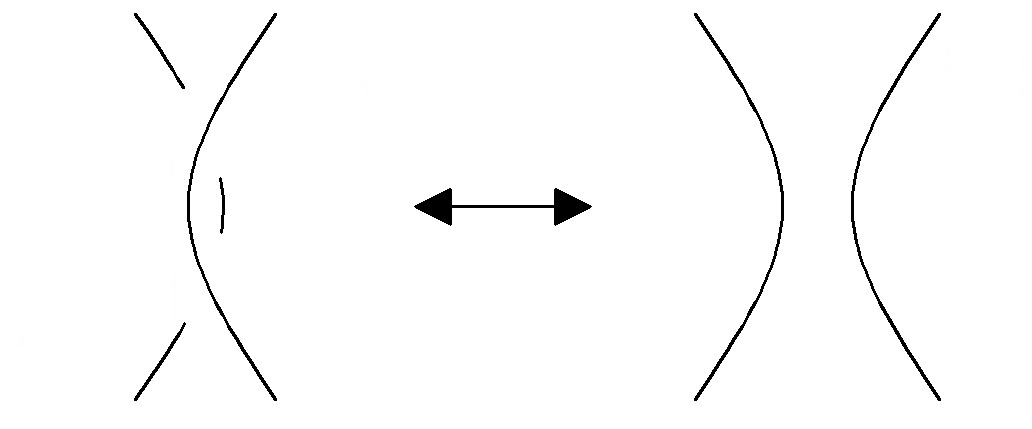
\includegraphics[scale=0.2]{1/pictures/R2}
% 		\end{center}
% 	\end{minipage}
	
% \item Trzeci ruch Reidemeistera: 

% 	\begin{minipage}{0.65\textwidth}
% 		\begin{center}
% 			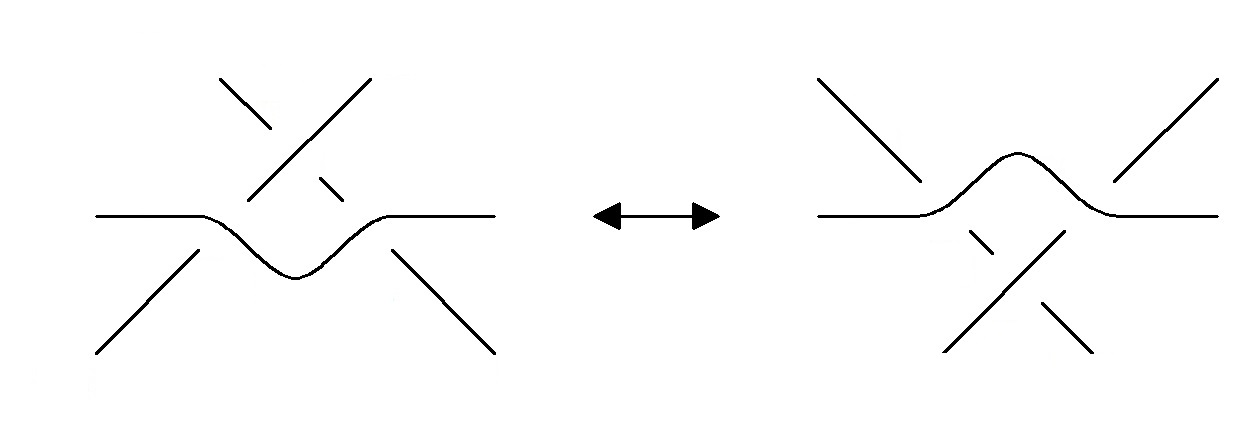
\includegraphics[scale=0.25]{1/pictures/R3}
% 		\end{center}
% 	\end{minipage}
	
% 	\end{enumerate}
 
% \end{definicja}

% \begin{definicja}
%  Dwa diagramy uważa się za równoważne, gdy za pomocą skończonej liczby ruchów Reidemeistera z jednego diagramu można otrzymać drugi.
% \end{definicja}

% \begin{twierdzenie}{(Reidemeister'a)}
% Dwa węzły są równoważne, wtedy i tylko wtedy, gdy ich diagramy są równoważne.
% \end{twierdzenie}

% \begin{proof}

% Załóżmy najpierw, że mamy dane węzły $J$ i $K$, oba te węzły mają regularny rzut na płaszczyznę, oraz węzeł $K$ można otrzymać z węzła $J$ przez pewien ciąg elementarnych deformacji.
% Ponieważ ten ciąg jest skończony, bez zmniejszenia ogólności możemy założyć, że węzeł $K$ powstaje z węzła $J$ w wyniku jednej elementarnej deformacji. Wystarczy więc pokazać, że 
% ta deformacja odpowiada ciągowi ruchów R na diagramie węzła $J$. 

% Rozważmy pojedynczą elementarną deformację węzła $J$ w sensie definicji \ref{wygoda}. Powiedzmy że $J = (v_1, \ldots, v_{i-1}, v_i, v_{i+1}, \ldots, v_n)$, oraz że 
% $K = (v_1, \ldots, v_{i-1}, v', v_{i+1}, \ldots, v_n)$. Ogólny przypadek na pierwszy rzut wydaje się być mocno skomplikowany. Opiszemy go za pomocą wielu podprzypadków, z którymi
% w prosty sposób potrafimy sobie poradzić. 

% Niech $C$ oznacza czworokąt $v_{i-1}, v_i, v_{i+1}, v'$, przez $o$ oznaczmy odcinek $vv'$. Przez $S$ oznaczmy zbiór skrzyżowań z wnętrza $C$ (jako podzbiór $\mathbb{R}^2$), 
% przez $W$ oznaczmy zbiór wierzchołków z wnętrza $C$, przez $P$ oznaczmy zbiór punktów przecięcia osi $o$ z łukami z wnętrza $C$. 
% Oczywiście zbiór $S\cup W\cup P$ jest skończony. Niech $A$ oznacza obraz tego zbioru przez rzut promienisty na $o$, to znaczy, jeśli dany punkt $p$ jest po tej samej stronie osi $o$, 
% co punkt $v_{i-1}$($v_{i+1}$), to rzutem promienistym punktu $p$ na $o$ nazwiemy rzutowanie na $o$ w kierunku prostej zawierającej odcinek $[p, v_{i-1}]$($[p, v_{i+1}]$). 
% Możemy założyć, że rzuty punktów z $S\cup W\cup P$ są parami różne, oraz że żadne skrzyżowanie ani wierzchołek nie leżą na osi $o$.
% Jeśli by tak nie było, możemy używając drugiego ruchu R odrobinę poprzesuwać skrzyżowania i miejsca przecięcia łuków z osią. 
% Niestety w przypadku, kiedy skrzyżowanie i wierzchołek znajdują się na prostej, wzdłuż której odbywa się rzutowanie, sytuacja jest nieco bardziej skomplikowana, co widać na poniższym
% rysunku.



% 	\begin{center}

% 	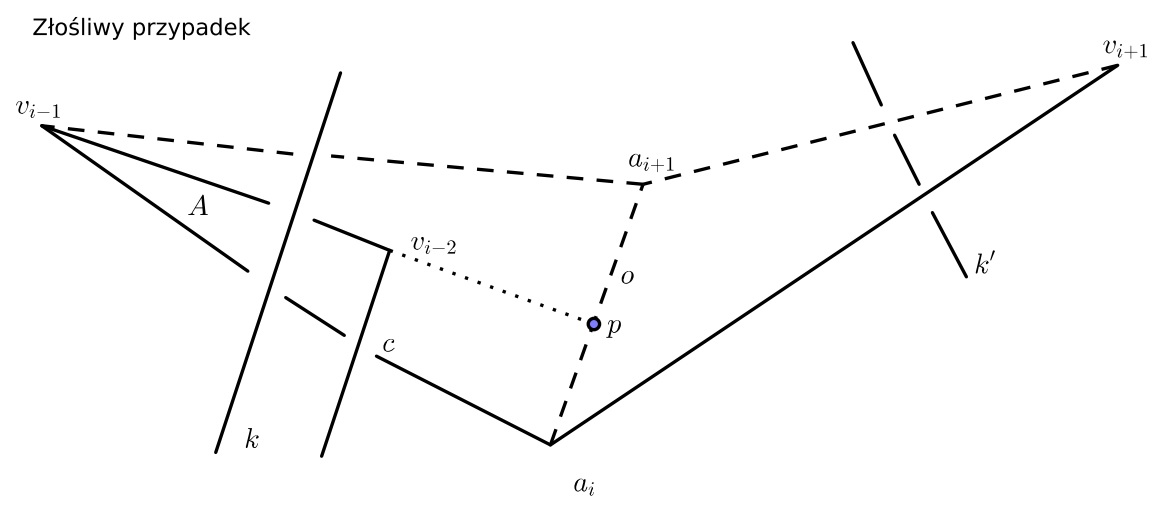
\includegraphics[scale=0.5]{1/pictures/bad.jpg}
% 	\end{center}


% Oczywiście łuków złośliwych w sensie złośliwości łuku $k$ może być więcej, niż jeden (bez zmniejszenia ogólności możemy założyć, że wewnątrz $C$ nie ma skrzyżowań - 
% to założenie będzie łatwo wynikać z dalszej części dowodu), ale będzie istniał taki, którego skrzyżowanie z $I_{i-1}$ będzie najbliżej wierzchołka $v_{i-2}$.
% Radząc sobie z tym delikwentem, oraz używając indukcji (skończonej), jesteśmy w stanie poradzić sobie z przypadkiem, kiedy złośliwych łuków jest dowolnie wiele. To jednak nie wyczerpuje
% wszystkich tego typu przypadków. Istnieje kilka podobnych (ale nie jest ich wiele, pamiętajmy, że $C$ ma być rozłączny z resztą węzła), np. łuk $k$ przechodzi pod czworokątem $C$, a odcinki $I_{i-2}, I_{i-1}$ przechodzą pod $k$. 
% Ponieważ wszystkie te przypadki są bardzo podobne, tu opiszemy tylko jeden, a resztę zostawiamy czytelnikowi jako nietrudne ćwiczenie.
% Aby poradzić sobie z przypadkiem przedstawionym na rysunku powyżej, należy najpierw łuk $k$ przenieść na drugą stronę skrzyżowania $c$ (trzeci ruch R), potem cofnąć wierzchołek $v_{i-2}$
% tak, żeby znajdował się bliżej wierzchołka $v_{i-1}$ niż łuk $k$ przed przesunięciem (tu nam pomoże drugi ruch R zastosowany parokrotnie), 
% następnie wrócić łuk $k$ na jego pierwotne miejsce (znów trzeci ruch R).
 

% Niech $B$ oznacza zbiór zrzutowanych punktów na oś $o$. Wprowadżmy na $o$ następującą relację porządku: $x < y\iff d(v_i,x) < d(v_i, y)$. Ustawmy zbiór $B$ rosnąco $x_1, x_2, \ldots, x_{l-1}$.
% Niech $v_i = a_0, a_1, a_2, \ldots, a_l = v'$ będzie ciągiem punktów, takim że $a_i\in o$, oraz $x_i < a_i < x_{i+1}$ w sensie wprowadzonego porządku. 
% Wystarczy zatem pokazać, że każdą z elementarnych deformacji przeprowadzających wierzchołek $v_i$ na $a_1$, wierchołek $a_1$ na punkt $a_2$, $\ldots$, 
% wierzchołek $a_{l-1}$ na punkt $a_l$ można uzyskać za pomocą sekwencji ruchów R, co prowadzi do rozbicia problemu na wiele mniejszych podprzypadków, których lista znajduje się
% poniżej.


% 	\begin{center}

% 	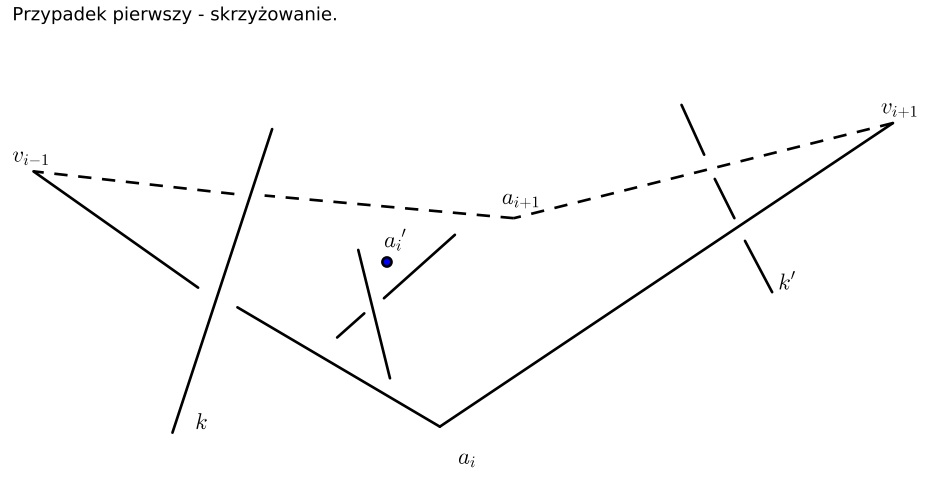
\includegraphics[scale=0.6]{1/pictures/cross.jpg}
% 	\end{center}

% Łuki skrzyżowania mogą przechodzić, albo oba nad bokami czworokąta $C$, albo oba pod bokami $C$, albo jeden może leżeć nad czworokątem, a drugi pod. Dwa pierwsze przypadki są oczywiste,
% radzimy sobie z nimi stosując trzeci ruch R, oraz w celach kosmetycznych drugi ruch R. Trzeci przypadek jest nieco trudniejszy, ale również główną rolę gra w nim trzeci ruch R. Po
% prostu można przenieść łuk, który przechodzi nad czworokątem $C$ na drugą stronę skrzyżowania łuku przechodzącego pod czworokątem $C$ i łuku $a_i v_{i-1}$, potem parokrotnie zastosować
% drugi ruch R a na koniec znów zastosować trzeci ruch R, żeby przenieść łuk, który ruszyliśmy na początku, na jego pierwotne miejsce.


% 	\begin{center}

% 	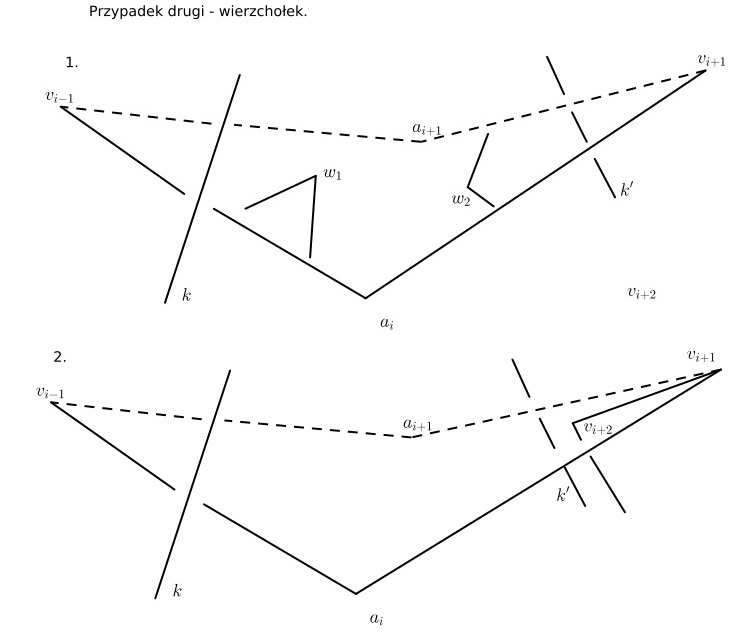
\includegraphics[scale=0.8]{1/pictures/vertex.jpg}
% 	\end{center}

	
% Podprzypadek pierwszy jest prosty, wystarczy zastosować drugi ruch R. Przypadek drugi wymaga nieco komentarza. 

% Żeby poradzić sobie z przypadkiem 2. należy zastosować pierwszy ruch R (wcześniej go nie stosowaliśmy) do pętli $a_iv_{i+1}v_{i+2}$. To nam pozwoli wyrzucić wierzchołek $v_{i+2}$ z 
% czworokąta $C$. Mamy też pewność, że efektem ubocznym tego ruchu nie będą żadne nowe skrzyżowania, ani wierzchołki, ani łuki przecinające oś $o$, zatem będziemy w stanie przenieść 
% wierzchołek $a_i$ na wierzchołek $a_{i+1}$. Na koniec, musimy wykonać operację odwrotną do tej, która wyrzuciła wierzchołek $v_{i+2}$ z czworokąta $C$, która sprawi, że $v_{i+2}$
% wróci na swoje pierwotne miejsce.


% 	\begin{center}

% 	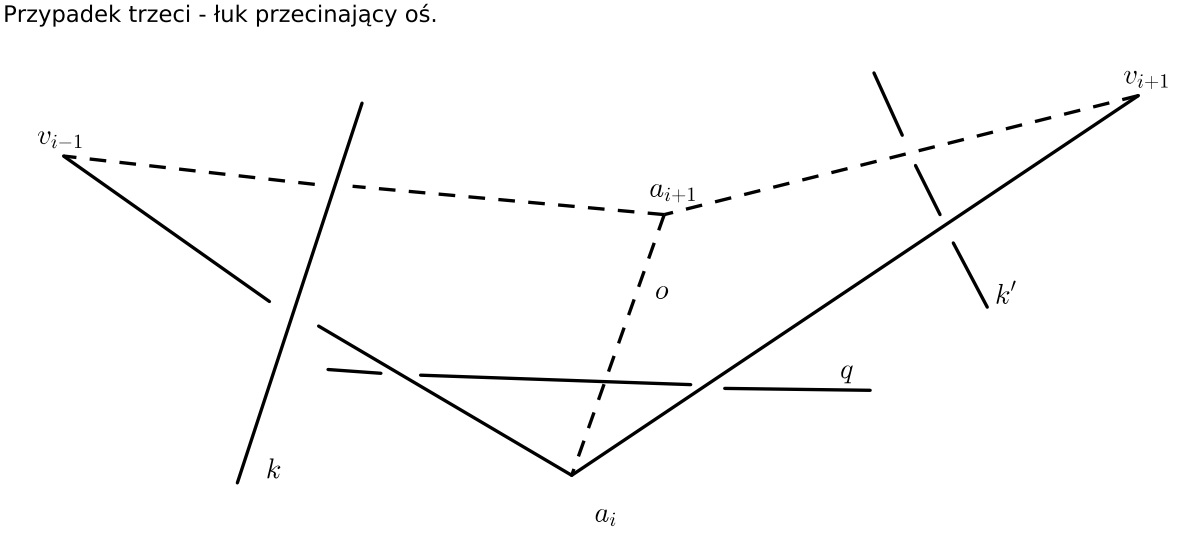
\includegraphics[scale=0.5]{1/pictures/axis.jpg}
% 	\end{center}

	
% Ten przypadek jest prosty, żeby przenieść wierzchołek $a_i$ na drugą stronę łuku $q$ wystarczy zastosować drugi ruch R. Przypadek, kiedy łuk $q$ przechodzi nad czworokątem $C$ jest analogiczny.

% Na koniec trzeba jeszcze pamiętać o naszym początkowym założeniu o tym, że rzuty są parami różne, i że żadne skrzyżowania, ani wierzchołki nie leżą na osi $o$. Jeśli potrzebowaliśmy
% lekko zmodyfikować diagram wyjściowego węzła, żeby to założenie było prawdziwe, musimy na koniec wykonać modyfikacje odwrotne, które oczywiście można uzyskać za pomocą ruchów R.

% W ten sposób zakończyliśmy szkic dowodu implikacji w jedną stronę. Implikacja w drugą stronę jest oczywista. 
	
% \end{proof}

\begin{definicja}
Węzeł to łamana w $\mathbb{R}^3$ bez samoprzecięć.
\end{definicja}